%% LyX 2.3.2-2 created this file.  For more info, see http://www.lyx.org/.
%% Do not edit unless you really know what you are doing.
\documentclass[12pt,english]{article}
\usepackage[latin9]{inputenc}
\usepackage[a4paper]{geometry}
\geometry{verbose,tmargin=4cm,bmargin=4cm,lmargin=4cm,rmargin=4cm}
\synctex=-1
\usepackage{color}
\usepackage{array}
\usepackage{float}
\usepackage{booktabs}
\usepackage{pmboxdraw}
\usepackage{amsmath}
\usepackage{amssymb}
\usepackage{graphicx}
\usepackage{setspace}
\usepackage[authoryear]{natbib}
\doublespacing

\makeatletter

%%%%%%%%%%%%%%%%%%%%%%%%%%%%%% LyX specific LaTeX commands.
%% Because html converters don't know tabularnewline
\providecommand{\tabularnewline}{\\}

\makeatother

\usepackage{babel}
\begin{document}
\title{\onehalfspacing{}Modeling How Macroeconomic Shocks Affect Regional Employment: Analyzing
the Brazilian Formal Labor Market using the Global VAR Approach}
\maketitle
\begin{abstract}
Assessing linkages across regions and how macroeconomic shocks spread
out across regions is not an easy task. We address the curse of dimensionality
using a global vector autoregressive methodology. Focusing on the
Brazilian labor market, identified and quantified how a shock in an
aggregate economic activity spreads out regionally and throughout
time. Another novelty is the use of information collected by the Brazilian
Bureau of Geography and Statistics to measure how regions are linked
by analyzing infrastructure linkages municipalities. We provide evidence
that macroeconomic shocks cause stronger effects on more developed
regions where formal labor market is better developed.
\end{abstract}
JEL codes: R11, E27, C23.

Key words: GVAR, cointegration, regional dynamics and labor market.

\pagebreak{}
\begin{doublespace}

\section{Introduction}
\end{doublespace}

\begin{doublespace}
\noindent \textcolor{black}{Macroeconomic shocks affect sectors and
regions with different intensities and delays. Population and economic
activities tend to cluster in specific areas due economies of scale
and agglomeration. The population tends to locate near the sea coast
compared with interior continental areas. Sector activities tend to
be concentrated in some areas or cities. Existence of a good economic
infrastructure such as roads, airports, ports, and telecommunications
facilities links regions economically and provides channels that can
spread out economic shocks among regions. Macroeconomic models tend
to disregard regional and spatial economic activity issues due to
either their aggregate nature bias or complexity of theme. However
for a specific region, it is important to understand how economic
activity variance can be decomposed into macroeconomic and idiosyncratic
factors.}

\noindent In the past years, time series data at disaggregated and
regional levels are becoming available. At the same time, efforts
have been made in econometric literature to model high-dimensional
problems. Two challenges must be faced to address interdependence
among regions, and linkages from regions to macroeconomic scenario.
The first is the curse of dimensionality. The second challenge involves
modeling the linkage between regions. 

\noindent \citet{chudik2011infinite} suggested two approaches to
handle the curse of dimensionality: (i) shrinkage of the parameter
space and (ii) shrinkage of the data. The authors dealt with the curse
of dimensionality by shrinking the parameter space as the number of
endogenous variables tends to infinity. In this configuration, the
infinite-dimensional vector autoregressive model could be well approximated
by a set of finite-dimensional small-scale models. Moreover, this
model can be estimated separately in a consistent manner, which is
the global vector autoregressive (GVAR) model proposed by \citet{pesaran2004modeling}.

\noindent Therefore, this study proposes a novel approach for dealing
with the curse of dimensionality when modeling the labor market: use
of the GVAR methodology to model the labor market at a regional level,
accounting for interdependence among regions as well as among global
macroeconomic variables. The GVAR methodology eliminates the curse
of dimensionality and provides a parsimonious model for the labor
market, and since the all variables are treated as endogenous, the
GVAR model allows the global variables to be affected by the regional
variables through a feedback channel.

\noindent We use information collected by the Brazilian Institute
of Geography and Statistics (IBGE)\footnote{Initials come from ``Instituto Brasileiro de Geografia e Estat�sticas''. }
that maps infrastructure and economic linkages across all municipalities
in Brazil to construct the weights used in GVAR to model interdependence
across regions. We do not restrict our analysis to neighborhood effects
on economic activity by constructing a measure of economic connections.

\noindent Focusing on the Brazilian labor market, the aim of study
is twofold. First, we want to model the link between an aggregate
macroeconomic variable and regional labor dynamics as well as accounts
for interdependence among Brazilian regions. To achieve that, a GVAR
methodology proposed by \citet{pesaran2004modeling} is used. Second,
we want to map how regional formal labor employment reacts to Brazilian
national economic activity. We employ monthly records of admissions
and discharges in the Brazilian formal regional labor market. The
period of the study is only 2004 to 2016 due to data constraints.
The model analysis led to the conclusion that the Brazilian Northeast
and South regions are the most elastic, whereas the North and Central
regions are less sensitive to macroeconomic shocks. The Southeast
region - the most developed in the country - is at the middle level.

\noindent This study is divided into sections as follows: section
2 is a brief literature review of previous works related to the purpose
of this study; section 3 presents the methodology; section 4 defines
the models used; section 5 describes the data with a brief description
of sources and characteristics; section 6 reports the results; and
section 7 contains final considerations. 
\end{doublespace}
\begin{doublespace}

\section{Literature Review}
\end{doublespace}

\begin{doublespace}
\noindent This section presents a brief literature review on the literature
that deals with spatial time series models and labor market. 

\noindent Firstly, focusing on the Brazilian labor market, \citet{oliveira2001flutuaccoes}
analyzed the fluctuations in the employment level of several Brazilian
states compared to national employment. The purpose of their study
was to verify whether it is possible to establish a long-term relationship
between state employment and nationwide employment. To achieve this
the authors applied a cointegration analysis, a methodology proposed
by \citet{engle1987co}, as well as the model of unrestricted error
correction as proposed by \citet{pesaran1996testing}.

\noindent The authors used a database that included a comprehensive
coverage of the labor market in the Brazilian states, using data from
the Annual Report on Social Information (RAIS)\footnote{ RAIS from the Portuguese Rela��o Anual de Informa��es Sociais.}
from 1985 through 1996. The results obtained from an Vector Error
Correction model were consistent with those obtained with Engle and
Granger method (\citet{engle1987co}). The results lead to the conclusion
that employment fluctuations in most states shares a common trend
with national employment level.

\noindent The hypothesis that the formal labor market presents a different
dynamics in Brazilian metropolitan and non-metropolitan areas was
tested by \citet{kretzmann2009flutuaccoes}. The goal of their study
was to analyze the fluctuations in the labor market of metropolitan
and non-metropolitan Brazilian areas. They used employment and unemployment
data from the Ministry of Labor and Employment through the General
Records of Employed and Unemployed Persons - CAGED\footnote{Initials comes from ``\textit{Cadastro Geral de Empregados e Desempregados}''
in Portuguese)} - using monthly data from 1996 through 2007. \citet{kretzmann2009flutuaccoes}
used cointegration analysis through the traditional method proposed
by Engle-Granger, as well as the method proposed by \citet{pesaran1996testing}.
The two methods produced the similar results, suggesting that the
metropolitan and non-metropolitan areas are not co-integrated.

\noindent None of these paper deals with the curse of dimensionality.
The authors opt to with pairs of series. The evidence that states
and national share a common trend highlight a possible channel linking
macro and regional dynamics. Evidence that metropolitan and non metropolitan
areas do not share a common trend may be explained by the fact that
neighborhood effects are not that relevant but when corrected by infrastructure
connections they may be. This hypothesis is investigated in this work. 

\noindent Secondly, \citet{pesaran2004modeling} introduced the Global
Vector Autoregressive (GVAR) methodology by means of a study that
modeled 11 different regions using data from 1979 through 1999. This
methodology was improved by \citet{dees2007exploring} with the collaboration
of the European Central Bank.

\noindent One of the first studies that applied GVAR to tackle interdependence
across regions is \citet{schanne2015global}. The author analyzed
the regional labor market in Germany with a focus on forecasting regional
labor markets. His study had two goals: the first one is to estimate
a the GVAR model, as proposed by \citet{pesaran2004modeling}. Second,
to use the developed GVAR model to construct a forecast for German
employment accounting for spatial effects.

\noindent The GVAR model allows both the analysis of strong cross-section
dependence and weak cross-section dependency. Consequently, \citet{schanne2015global}
concludes that the data indicate semi-strong cross-section dependence
and has consistent results since Germany is a polycentric economy,
in contrast with the United Kingdom or France (places where there
are clearly dominant regions). The final model used in his study is
a basic GVAR specification, which is a model in first differences
without imposing cointegration relations, and did not include a dominant
region.

\noindent In his forecasting experiment, \citet{schanne2015global}
estimated the basic GVAR model and GVAR models with leading indicators.
The author used these models as a predictive forecasting tool for
three and twelve months ahead -- forecasting the level of unemployment
in the regional divisions according to the federal employment agency
of Germany. For comparison purposes, each indicator was estimated
by a VAR in differences and a VAR in level. The accuracy of the prediction
was evaluated by comparing the absolute mean of prediction errors
(percentage) and by the Diebold-Mariano test (\citet{DM1995}). Finally,
\citet{schanne2015global} concluded that there is significant improvement
in the accuracy of predictions when considering the interdependence
between regions, emphasizing that the degree of improvement depends
on the variables and horizon. 
\end{doublespace}
\begin{doublespace}

\section{Methodology}
\end{doublespace}

\begin{doublespace}
\noindent This section presents and describes the GVAR methodology,
which is the main methodology used in this study. It is assumed that
the reader is familiar with the VAR methodology and VECM as well as
their terminologies. 

\noindent \citet{chudik2011infinite} considered the curse of dimensionality
in the case of large linear dynamic systems. To deal with the curse,
they proposed to shrink the parameter space in the limit as the number
of endogenous variables tends to infinity. They showed that by shrinking
the parameter space, the infinite-dimensional VAR could be well approximated
by a set of finite-dimensional small-scale models that can be consistently
estimated separately, which is in the spirit of the GVAR models proposed
in \citet{pesaran2004modeling}. Therefore, \citet{chudik2011infinite}
concluded that the GVAR approach can be used as an approximation to
an nfinite dimension vector autoregressive model (IVAR) featuring
all macroeconomic variables. This is true for stationary models as
well as for systems with variables integrated of order one.

\noindent The GVAR model is a compact model that combines individual
VECMs in which domestic variables are related to individual-specific
foreign variables in a consistent manner. 
\end{doublespace}
\begin{doublespace}

\subsection{Global vector autoregressive model}
\end{doublespace}

\begin{doublespace}
\noindent The GVAR methodology was originally proposed by \citet{pesaran2004modeling}
as a practical approach to construct a coherent global model. In the
traditional VAR methodology, an unrestricted VAR(p) model with \textit{k}
endogenous variables covering \textit{N} countries has a large number
of unknown parameters of the order $(k\centerdot N)^{2}p+kN$ in the
mean plus $\frac{(k\centerdot N+1)kN}{2}$ in the variance, thus requiring
a parsimonious solution. Therefore, the authors proposed the use of
a model wherein, first, the error correction models specific to each
region are estimated, with the domestic macroeconomic variables related
to the corresponding foreign variables, and second the models from
each region are combined to generate forecasts for all variables.
In short, the GVAR model combines the VECM models of each region,
so that domestic variables are related to regionally specific foreign
variables in a consistent manner. Therefore, the model can consider
the interdependencies between economic regions in the analysis.

\noindent Subsequently \citet{dees2007exploring} improved the GVAR
model with the cooperation of the European Central Bank. This version
of the GVAR model included 26 countries (covering 90\% of world production),
with the Euro area being considered as one sole economy with estimates
from 1979 to 2003. The version of GVAR model used in this study is
based on that of \citet{dees2007exploring}.

\noindent The GVAR model can be summarized as a two-step procedure.
In the first step, specific models of each region are estimated that
are conditioned to the external influences of other regions. That
is, the models are represented as VAR models, which have domestic
variables and foreign variables, the latter being treated as weakly
exogenous.\footnote{See \citet{engle1983exogeneity} for a definition.}
In the second step, the VAR models of each region are grouped into
one single GVAR model. The GVAR model, as well as any VAR model, can
be used for analyzing shocks in the economy and making predictions.
\end{doublespace}
\begin{doublespace}

\subsubsection{Specific models for each region}
\end{doublespace}

\begin{doublespace}
\noindent For the specific models used in the first stage of the GVAR
methodology, consider a panel with $N$ elements, each element showing
$k_{i}$ variables observed during periods $t=1,2,\cdots,T$. Within
this panel structure the following variables are defined: $x_{i,t}$
as a vector $k_{i}\times1$ of domestic variables for element \textit{i}
in period \textit{t}; $x_{it}^{*}$ as a vector $k^{*}\times1$ of
foreign variables; and $u_{i,t}$ as an error vector. Thus, following
the notation of \citet{chudik2016theory}, the specific models of
each element consist of a set of domestic and foreign variables. Specifically,
for any $i$ element:

\noindent 
\begin{equation}
x_{i,t}=a_{i0}+a_{i1}t+\sum\limits _{j=1}^{p_{i}}\Phi_{ij}x_{i,t-j}+\Lambda_{i0}x_{i,t}^{*}+\sum\limits _{l=1}^{q_{i}}\Lambda_{il}x_{i,t-l}^{*}+u_{i,t},
\end{equation}

\noindent where $\Phi_{ij}$ is an array of lag coefficients for lag
$j$ associated with domestic variables, and $\Lambda_{il}$ is an
array of lag coefficients for lag $l$ associated with foreign variables.

\noindent The GVAR model treats foreign variables as weights averages
of the domestic variables of each corresponding element, and the weights
are specific to each unit. Therefore, the foreign variables of each
element \textit{i} can be computed as weights of the domestic variables
of other units in the panel. $W_{ij}$ is a weighting matrix, where
$j=1,2,\cdots,N$ is defined as a set of weights with the following
characteristics: $W_{ii}=0$ and $\sum_{j=1}^{N}W_{ij}=1$. Thus,
the foreign variables can be defined as

\noindent 
\begin{equation}
x_{i,t}^{*}=\sum\limits _{j=0}^{N}W_{ij}x_{jt}.\label{eq:W}
\end{equation}

\noindent The weights are predetermined and used to capture the importance
of region $j$ for the economy of region $i$.

\noindent From the domestic and foreign variables estimated from the
weighting previously mentioned, VECMs are estimated separately for
each region, considering that in the VECMs, the foreign variables
$x_{i,t}^{*}$ are treated as weakly exogenous. The use of the VECMs
allows cointegration between domestic variables and between domestic
and foreign variables.
\end{doublespace}
\begin{doublespace}

\subsubsection{Global model}
\end{doublespace}

\begin{doublespace}
\noindent Although estimation is performed individually, element by
element, the GVAR model is solved by considering all variables as
endogenous to the system. Thus, from the specific model of each element,
$Z_{i,t}$ is defined as

\noindent 
\begin{equation}
Z_{i,t}=\begin{bmatrix}x_{i,t}\\
x_{i,t}^{*}
\end{bmatrix},\label{eq:ZZ}
\end{equation}

\noindent Using (\ref{eq:W}) in (\ref{eq:ZZ}) it is possible to
obtain

\noindent 
\begin{equation}
A_{i0}Z_{i,t}=a_{i0}+a_{i1}t+\sum_{l=1}^{p}A_{il}Z_{i,t-l}+\varepsilon_{i,t},\label{eq:AZ}
\end{equation}

\noindent where $p=\max_{i}\{p,q_{i}\}$, $A_{i0}=[\begin{array}{cc}
I_{k_{i}} & -\Lambda_{i0}\end{array}]$, and $A_{il}=[\begin{array}{cc}
\Phi_{il} & \Lambda_{il}\end{array}]$ for $l=1,2,\cdots,p$. Moreover we define $\Phi_{il}=0$ for $l>p_{i}$
and $\Lambda_{il}=0$ for $l>q_{i}$.

\noindent Let $x_{t}=[x_{0,t}^{'},x_{1,t}^{'},\cdots,x_{N,t}^{'},]^{'}$
be a vector $k\times1$ of all the variables in the panel, where $k=\sum_{i=1}^{N}k_{i}$
. $W_{i}$ can be defined as a matrix of dimension $(k_{i}+k_{i}^{*})\times1$
of known constants defined in terms of the individual weights $W_{ij}$.
Therefore, variables of the specific models are defined as a function
of $x_{t}$.

\noindent 
\begin{equation}
Z_{i,t}=W_{i}x_{t}
\end{equation}

\noindent Using this identity, the individual models can be written
as

\noindent 
\begin{equation}
A_{i0}W_{i}x_{t}=a_{i0}+a_{i1}t+\sum_{l=1}^{p}A_{il}W_{i}x_{t-l}+\varepsilon_{i,t},
\end{equation}

\noindent It is possible to combine the new individual models into
one single model, and this can be done by \textquotedblleft stacking
up\textquotedblright{} each model in a large-scale VAR.

\noindent 
\begin{equation}
G_{0}x_{t}=a_{0}+a_{1}t+\sum_{l=1}^{p}G_{l}x_{t-l}+\varepsilon_{t},\label{eq:g0xt}
\end{equation}

\noindent where

\noindent 
\[
\begin{array}{ccccc}
G_{0}=\begin{bmatrix}A_{00}W_{0}\\
A_{10}W_{1}\\
\vdots\\
A_{N0}W_{N}
\end{bmatrix}, & G_{1}=\begin{bmatrix}A_{0l}W_{0}\\
A_{1l}W_{1}\\
\vdots\\
A_{Nl}W_{N}
\end{bmatrix}, & a_{0}=\begin{bmatrix}a_{00}\\
a_{10}\\
\vdots\\
a_{N0}
\end{bmatrix}, & a_{1}=\begin{bmatrix}a_{01}\\
a_{11}\\
\vdots\\
a_{N1}
\end{bmatrix}, & \varepsilon_{t}=\begin{bmatrix}\varepsilon_{0,t}\\
\varepsilon_{1,t}\\
\vdots\\
\varepsilon_{N,t}
\end{bmatrix},\end{array}
\]

\noindent Since the $G_{0}$ matrix is a non-singular matrix, which
depends only on the estimated parameters and the link matrix $W_{i}$,
it is possible to rewrite equation (\ref{eq:g0xt}) as

\noindent 
\begin{equation}
x_{t}=b_{0}+b_{1}t+\sum_{i=1}^{p}F_{i}x_{t-i}+\epsilon_{t},
\end{equation}

\noindent where

\noindent 
\[
\begin{array}{c}
F_{i}=G_{0}^{-1}G_{i},\\
b_{0}=G_{0}^{-1}a_{0},\\
b_{1}=G_{0}^{-1}a_{1},\\
\epsilon_{t}=G_{0}^{-1}\varepsilon_{t},
\end{array}
\]

\noindent Hence, the global model, which consists of a set of individual
models from each region, can be solved recursively. With that, it
is possible to consistently determine the coefficients of the model.
\end{doublespace}
\begin{doublespace}

\subsubsection{Dominant unit model}
\end{doublespace}

\begin{doublespace}
\noindent Global VAR is based on the hypothesis of weak exogeneity
(\citep{engle1983exogeneity}). If this hypothesis fails for one or
more regions, these regions must be modeled jointly. In spatial analysis,
it is possible that some important regions affect others in a specific
form. This information must be included in the model. Therefore, vector
$\omega_{t}$ of common variables and its lagged values augment each
specific model. So, each element of the model can be stated as

\noindent 
\begin{equation}
x_{i,t}=a_{i0}+a_{i1}t+\sum_{j=1}^{p_{i}}\Phi_{ij}x_{i,t-j}+\Lambda_{i0}x_{i,t}^{*}+\sum_{l=1}^{q_{i}}\Lambda_{il}x_{i,t-l}^{*}+D_{i0}\omega_{t}+\sum_{l=1}^{s_{i}}\Psi_{il}\omega_{t-l}+u_{i,t},
\end{equation}

\noindent The marginal model for the dominant variables can be estimated
with the feedback effects from $x_{t}$, or not. The feedback from
the variables in the GVAR model are captured via cross-section averages,
and this is done by augmenting the dominant unit model with lags of
$x_{\omega t}^{*}$.

\noindent 
\begin{equation}
\omega_{t}=\sum_{l=1}^{p_{\omega}}\Phi_{\omega l}\omega_{t-l}+\sum_{l=1}^{q_{\omega}}\Lambda_{\omega l}x_{i,t-l}^{*}+\eta_{\omega t}
\end{equation}

\noindent Different lag orders for the dominant variables ($p_{\omega}$)
and cross-section averages ($q_{\omega}$) could be considered. It
is worthy to point out that contemporaneous values of foreign variables
do not feature in the equation.
\end{doublespace}
\begin{doublespace}

\subsection{Regional weights}
\end{doublespace}

\begin{doublespace}
\noindent Finally, the number of connections between regions were
obtained from \citet{ibge}. This work aims to determine economic
linkage among municipalities in Brazil. The study analyzed not only
regular transport links, such as those that go to the urban centers,
but also the main destinations of the residents to obtain products
and services, such as general goods, education, airport travel, and
health services. The acquisition of agricultural inputs and destination
of the agricultural products were also analyzed in the study. The
main result of the research is a Brazilian urban network map that
connects all 5,564 Brazilian municipalities. This map contains the
hierarchy of the urban network and the regions of influence of each
urban center.

\noindent A chart indicating the connections between all Brazilian
cities is constructed by merging the links provided in the urban network
framework, which are the main links between municipalities, with the
links regarding airport connections, shopping destinations, education,
health services, and recreation activities. 

\noindent Since every city belongs to a mesoregion, the links between
mesoregions are also determined with the following characteristics:
if the two cities are within the same region then the link between
them is an internal link; if the two cities are in different mesoregions,
then the link between them is a connection between the two mesoregions.

\noindent As mentioned earlier, the weight matrix is a function of
the number of connections between regions; however at this point,
it is worth mentioning that some connections are more important than
others. Moreover, since the measurement of importance for each connection
between each region is unfeasible, an equal weight to all connections
is assumed, resulting in a linear function, which is the average.

\noindent The weight matrix to region \textit{i} can then be determined
by the number of connections to other regions divided by its total
number of connections. Therefore, the weight vector for each region
is determined as

\noindent 
\begin{equation}
W_{i}=\frac{\begin{bmatrix}C_{i1} & \cdots & C_{iN}\end{bmatrix}}{\sum_{j=1}^{N}C_{ij}},\label{eq:dddd}
\end{equation}

\noindent where $C_{ij}$ is the number of connections that originated
at region $i$ and have region $j$ as destination, keeping in mind
that connections within the same region ($i=j$), also called internal
links, have a zero weight ($C_{ii}=0$).

\noindent One most important step in GVAR methodology is the construction
of the weight matrix. In Pesaran\textquoteright s initial work, the
weight matrix is defined by country-specific trade weights. In fact,
the weight matrix $W_{i}$ is designed to capture the importance of
all other regions for region \textit{i} (\citealp{di2013gvar}). So,
to determine the weight matrix it is necessary to determine the importance
of each region in respect to every other region.

\noindent Focusing on the labor market, to determine the importance
of a region to another is to determine the importance of one labor
market to another labor market. Each region has its own labor market
with firms and workers, and since firms cannot change markets, it
is the workers that freely change markets. In other words, a worker
can look for a job in other regions, but a firm must attract workers
from other regions to its own market. Consequently, for a worker to
commute to another region, there must be a connection between these
regions.

\noindent The connections between regions go beyond neighborhood effects
in an integrated economy. There are many other channels such as physical
infrastructure that allow workers to commute (by car, by train, by
plane, etc.) to another region. Therefore, regions with higher connections
are more important than regions with fewer connections to model a
specific unit. 

\noindent Consequently, the importance of region $j$ to region $i$
will be a function of the connections between them, and the weight
matrix will be a based on the number of connections between the regions. 
\end{doublespace}
\begin{doublespace}

\section{Database Description and Model Specification }
\end{doublespace}

\begin{doublespace}
\noindent The labor market interacts with the macroeconomic environment
through many channels. One of these channels is the level of economic
activity. Industrial production is used as a proxy to economic activity.
It is highly correlated to the gross domestic product (GDP) but available
at a higher frequency level. The first is available quarterly whereas
the latter is available monthly.

\noindent Finally, an attempt to model the Brazilian labor market
at the municipality level was made but then discarded. Brazil had
a total of 5,564 municipalities in 2005 according to IBGE. This government
institute grouped municipalities into 137 mesoregions and 27 states.
Many municipalities were merged or split, and thus it is difficult
to construct a long time series. Therefore, we opt to work at the
mesoregional level.
\end{doublespace}
\begin{doublespace}

\subsection{Database}
\end{doublespace}

\begin{doublespace}
\noindent Table \ref{tab:table1} contains a detailed description
of the data sources. The following section provides a brief description
of the data used in this study as well as their sources and frequency.

\noindent \textless Insert Table \ref{tab:table1} about here\textgreater{}

\noindent Data for the Brazilian industrial production were obtained
from IBGE. The employment and unemployment records, which indicate
the workers admitted to and discharged from the labor market, were
obtained from CAGED.\footnote{Initials come from ``Cadastro Geral de Empregados e Desempregados''. }
The data were obtained at the municipality level and grouped by mesoregions.
The frequency of the data is monthly starting from January 2004 to
December 2016.

\noindent The mesoregions' definitions, as well as information on
the total population, microregions, mesoregions, states, and their
designation codes, were obtained from IBGE as reported in 2015.
\end{doublespace}
\begin{doublespace}

\subsection{Descriptive statistics}
\end{doublespace}

\begin{doublespace}
\noindent Table \ref{tab:table2} shows descriptive statistics for
the industrial production as well as the admitted and disconnected
series for mesoregions that contain the cities of S�o Paulo, Rio de
Janeiro, and Brasilia - three of the most important cities in Brazil.
The descriptive statistics for all the regions can be found in the
appendices.

\noindent \textless Insert Table \ref{tab:table2} about here\textgreater{}

\noindent All models were estimated using MatLab software R2016b and
GVAR Toolbox 2.0. The following MatLab add-ons were installed during
the estimation of the models: Mapping Toolbox version 4.4, Econometrics
Toolbox version 3.5, Optimization Toolbox version 7.5, and Statistics
and Machine Learning Toolbox version 11.0. 
\end{doublespace}
\begin{doublespace}

\subsection{Global vector autoregressive model specification}
\end{doublespace}

\begin{doublespace}
\noindent The objective of this study is to use the GVAR methodology,
as described in the previous section, to assess the Brazilian labor
market model. Each Brazilian mesoregion will be a GVAR unit.

\noindent Since the labor market model consists of workers admitted
to and discharged from the labor market, the specific model for each
mesoregion will contain information of those admitted to and discharged
from the labor market in period \textit{t} for that region. Therefore,
for each mesoregion \textit{i} a vector $x_{it}$ can be defined as

\noindent 
\begin{equation}
x_{i,t}=\begin{bmatrix}Adm_{i,t}\\
Dis_{i,t}
\end{bmatrix},
\end{equation}

\noindent where $Adm_{i,t}$ is the number of workers admitted (employment
flow) to the labor market in period $t$ in region $i$, and $Dis_{i,t}$
is the number of workers disconnected (unemployment flow) from the
labor market in period $t$ in region $i$.

\noindent Each region experiences influences from other regions. Using
the GVAR methodology, the foreign variables are defined as a vector
$x_{i,t}^{*}$ as follows:

\noindent 
\begin{equation}
Adm_{i,t}^{*}=\sum_{j=1}^{N}W_{ij}Adm_{j,t},
\end{equation}

\noindent 
\begin{equation}
Dis_{i,t}^{*}=\sum_{j=1}^{N}W_{ij}Dis_{j,t},
\end{equation}

\noindent 
\begin{equation}
x_{i,t}^{*}=\begin{bmatrix}Adm_{i,t}^{*}\\
Dis_{i,t}^{*}
\end{bmatrix},
\end{equation}

\noindent where $W_{ij}$ is a link matrix that captures how much
region $j$ influences region $i$; $Adm_{i,t}^{*}$ is the influence
on region $i$ of the number of workers admitted to the labor market
in other regions in period $t$; and $Dis_{i,t}^{*}$ is the influence
in region $i$ of the number of workers disconnected from the labor
market in other regions in period $t$;

\noindent The specific models are defined with unrestricted intercepts
and no trend coefficients. It is worth mentioning that even though
a deterministic trend is not included in the model, the levels of
the domestic variables may be trended due to the drift coefficients.

\noindent 
\begin{equation}
x_{i,t}=a_{i0}+\sum_{j=1}^{k_{1,i}}\Phi_{ij}x_{i,t-j}+\Lambda_{i0}x_{i,t}^{*}+\sum_{l=1}^{k_{2,i}}\Lambda_{il}x_{i,t-l}^{*}+u_{i,t}
\end{equation}

\noindent where $k_{1,i}$ and $k_{2,i}$ are the lag order for the
domestic variables and foreign variables respectively. The model is
defined with a maximum two lag order for domestic and foreign variables,
where the lag selection for each region will be done by the GVAR Toolbox
using the Akaike information criteria. 
\end{doublespace}
\begin{doublespace}

\subsection{Macroeconomic dynamics}
\end{doublespace}

\begin{doublespace}
\noindent In the GVAR model, macroeconomic variables are treated as
common variables and modeled in a dominant unit. Therefore, the dominant
unit of the GVAR model will contain the log level of the Brazilian
industrial production defined by the vector $\omega_{t}$, with a
feedback variable from the regions through the aggregate values of
employment and unemployment. So, the dominant unit will be a univariate
model defined in first differences with a trend included in the levels,
and it can be expressed as

\noindent 
\begin{equation}
\omega_{t}=\begin{bmatrix}\log(IndProd_{t})\end{bmatrix},
\end{equation}

\noindent 
\begin{equation}
\Delta\omega_{t}=\Phi_{\omega0}+\sum_{l=1}^{k_{1}}\Phi_{\omega l}\Delta\omega_{t-l}+\sum_{l=1}^{k_{2}}\Lambda_{\omega l}\Delta x_{i,t-l}^{*}+\eta_{\omega t},
\end{equation}

\noindent where $\Delta x^{*}$ is the feedback variable containing
the aggregate values of employment and unemployment from all regions;
$k_{1}$ and $k_{2}$ are the lag orders for the global variable (industrial
production) and feedback variables, respectively. The maximum lag
order is defined as three for both the global variable and feedback
variables, where the lag selection for each variable will be set by
the GVAR Toolbox using Akaike information criteria. 
\end{doublespace}
\begin{doublespace}

\section{Results}
\end{doublespace}

\begin{doublespace}
\noindent Modeling a system such as the Brazilian labor market at
the mesoregion level is naturally subject to considerable uncertainties.
There are many choices to be made for each individual mesoregion model,
for example, about the variables to be included in the specific models,
lag order of the domestic variables, lag order of the foreign variables,
number of cointegrating relations, and whether to impose long-run
and short-run restrictions on the parameters.

\noindent As explained earlier, the GVAR model comprises several specific
models, solved in a two-step process. The model is defined using the
data for admissions and discharges for every mesoregion as well as
the weight matrix defined previously. All regions were set to be affected
by the foreign variable and dominant unit. 

\noindent The final model was estimated using the GVAR automatic lag
selection with the Akaike information criterion and a maximum lag
order of two for domestic as well as foreign variables. A total of
137 models were specified. Lags for domestic variables were set to
two in 98 models and to one in the other 39 models. The lags for foreign
variables were set to two in 91 models and to one in the other 46
models.

\noindent Existence of cointegration among variables was investigated
using an automated procedure of GVAR Toolbox 2.0. All individual models
had the deterministic components treated as an unrestricted intercept
and no trend in the error correction models. Out of the 137 estimated
models, nine were specified with one cointegration relationship, and
128 models were specified with two cointegration relationships.

\noindent The GVAR model determines a model for each region considering
foreign effects as well as effects from the variables in the dominant
unit model. With no overidentifying restrictions imposed, the final
model proved to be stable with 815 eigenvalues lying inside the unit
circle, 10 of which were lying on the unit circle. 
\end{doublespace}
\begin{doublespace}

\subsection{Forecast exercise}
\end{doublespace}

\begin{doublespace}
\noindent Using the GVAR methodology, it is possible to estimate the
dynamic response of unemployment and employment in each region, considering
not only the industrial production but also the interdependence of
each region. With the use of conditional forecasts, it is possible
to evaluate the behavior of the labor market in response to a change
in the global economy, which in our case is represented by the industrial
production. Therefore, a series of conditional forecasts for different
growth scenarios of industrial production were made to assess the
impact of the industrial production on the labor market. The series
of conditional forecasts of the labor market consist of a base scenario
and several other growth scenarios for the Brazilian industrial production.

\noindent The baseline scenario for industrial production growth will
have 0\% growth coefficient over the last year in the series, in this
case, 2016. The other growth scenarios on the set will have 2\% growth
coefficient, 4\% growth coefficient, 6\% growth coefficient, and 8\%
growth coefficient over the last year.

\noindent The industrial production growth is determined by applying
the annual growth coefficient in each month compared with that of
the last year. In other words, a 2\% growth coefficient means a 2\%
grow in January 2016 compared to January 2017 and so on. All the scenarios
were analyzed over an eight-year forecast.
\end{doublespace}
\begin{doublespace}

\subsubsection{Forecast, net employment, and accumulated employment}
\end{doublespace}

\begin{doublespace}
\noindent ``Net employment gain'' is defined as the difference between
admissions minus discharges. In addition \textquotedblleft total net
employment mesoregion gain\textquotedblright{} is defined as the sum
of the net employment gain for every municipality of the mesoregion.
Consequently, as the forecast exercise started in January 2017, the
cumulative employment gain is the sum of all the previous \textquotedblleft total
net employment\textquotedblright{} until that year. The total cumulative
employment is an aggregate of all mesoregions and can be used to evaluate
how the Brazilian labor market will behave in different macroeconomic
scenarios in terms of changes in stocks of employment. (Figure \ref{fig: fig-1})

\noindent \textless Insert Figure \ref{fig: fig-1} about here\textgreater{}

\noindent From 2015 through 2016, the total net employment gain is
-3 million because Brazilian economy was facing a deep recession.
Taking December 2016 as reference, the baseline forecasts reveal that
a 0\% annual growth for industrial production would imply a great
loss of formal employment. If industrial production starts to recover
at the rate of 2\% annual growth, then the net gain will become positive
only about September of 2021. At the end of the forecast horizon period,
a cumulative gain of 2.5 million net jobs will be created. A 4\% annual
growth in the industrial production would cause significant improvement
to the cumulative net employment gain with the first positive net
gain of the series occurring in September 2017, and the cumulative
gain of employment will be 6.5 million by the end of 2024. For 6\%
and 8\% annual growth, cumulative gain will become positive in June
2017, and it will have a value of 10.5 million and 14.5 million, respectively,
by the end of the forecast period. It is worth mentioning that 4\%
annual growth in the industrial production would compensate for the
Brazilian cumulative net employment deficit from 2015 to 2016 only
in July 2022. 
\end{doublespace}
\begin{doublespace}

\subsection{Industrial production elasticity by region}
\end{doublespace}

\begin{doublespace}
\noindent The net employment defined in the last section can be interpreted
as the variation on the total employment level. To normalize the value
we divide each variable by total population of each mesoregion. This
gives an idea about the dynamics of each region. It would be better
to have an estimate of labour force, but this is not available. Therefore,
changes in the employment rate used in this study are a proxy of employment
rate creation.

\noindent Since the GVAR methodology allows for a forecast for each
region, it is possible to map changes of the employment rate for every
region, where the cumulative changes are the sum of all previous variations.
Therefore, it is possible to evaluate how a change in the industrial
production affects the labor market in each region; in other words,
it is possible to establish the employment elasticity with respect
to the industrial production. (Figure \ref{fig: fig-2})

\noindent \textless Insert Figure \ref{fig: fig-2} about here\textgreater{}

\noindent Data on each mesoregion are grouped into five Brazilian
regions: North, Northeast, Southeast, South and Centralwest. Taking
the IBGE's estimated population for 2016 as the total population,
and 0\% growth as a base scenario, it is possible to obtain the industrial
production elasticity of employment for each major region over an
eight-year forecast period. Considering a 2\% annual growth in the
industrial production, the South region is the most sensitive with
0.18 elasticity; the second most sensitive region is the Northeast
with 0.15 elasticity. The Southeast region has 0.10 elasticity, while
the least sensitive major regions are the North and Centralwest, each
with 0.06 elasticity.

\noindent This indicates that the Northeast and South regions have
higher elasticity, being strongly affected by changes in industrial
production. The Southeast region, which is the most developed, has
intermediate elasticity. This is probably due to the high development
level of the region, making its marginal gain not as high as in the
Northeast and South regions.

\noindent Although previous analysis was conducted in macroregions,
the GVAR methodology allows us to conduct the same analysis at a more
in-depth level. Since the GVAR equations are solved for every region,
we can evaluate elasticity for not only the state but also for every
mesoregion.

\noindent Figure \ref{fig: fig-3} shows the estimated employment
rate change for the Southeast region, the most developed in the country.
Using 0\% growth as a base scenario, elasticity for the states of
Minas Gerais, Esp�rito Santo, Rio de Janeiro, and S�o Paulo are estimated.
Again, considering a 2\% annual growth in industrial production, Rio
de Janeiro is the most sensitive state with 0.19 elasticity, followed
by Esp�rito Santo with a 0.09 elasticity. Minas Gerais and S�o Paulo
are estimated to have elasticity of 0.07 and 0.08, respectively. 

\noindent \textless Insert Figure \ref{fig: fig-3} about here\textgreater{}

\noindent As mentioned earlier, with the GVAR model, it is possible
to evaluate every region in a more in-depth analysis. Since listing
all 137 regions' estimated elasticity would be impractical, the region
of S�o Paulo metropolitan area (one of the most important in the country)
is compared with four other randomly selected regions: Goi�s Central
region, Borborema region, Jequitinhonha region, and Porto Alegre metropolitan
area. Goi�s Central region is the most rich and densely populated
mesoregion of the Goi�s state, with 3.1 million inhabitants. The mesoregion
of Borborema is dry land, with approximately 310,000 inhabitants.
The Jequitinhonha Valley region is known for its low social indicators.
It has 731,000 inhabitants. Porto Alegre metropolitan area is an important
region in the South and its economy is strongly influenced by the
industrial sector 5 million inhabitants.

\noindent Figure \ref{fig: fig-4} shows the estimated elasticity
for the regions. As previously mentioned, 0\% growth is used as a
base scenario for the elasticity. With the scenario of 2\% annual
growth in industrial production, Porto Alegre is the most sensitive
mesoregion with 0.19 elasticity, followed by S�o Paulo with 0.16 elasticity.
The Goi�s central area has a moderate elasticity with a value of 0.07.
Lastly, the Borborema and Jequitinhonha mesoregions proved to be very
inelastic, with only 0.02 elasticity. 

\noindent \textless Insert Figure \ref{fig: fig-4} about here\textgreater{}

\noindent The most populated mesoregions in Brazil are S�o Paulo metropolitan
area, Rio de Janeiro metropolitan area, Belo Horizonte metropolitan
area, Porto Alegre metropolitan area, and Salvador metropolitan area.
According to IBGE in 2017, Rio de Janeiro metropolitan area has approximately
12.9 million inhabitants, and Belo Horizonte metropolitan area has
approximately 6.7 million inhabitants, and Salvador metropolitan area
has around 4.7 million inhabitants.

\noindent Figure \ref{fig: fig-5} shows the estimated elasticity
for the most populated mesoregions in Brazil. As before, 0\% growth
is used as a base scenario for the elasticity. With the scenario of
2\% annual growth in industrial production, the metropolitan areas
of Rio de Janeiro and Porto Alegre are the most sensitive mesoregions
with 0.19 elasticity. Belo Horizonte and S�o Paulo have elasticity
of 0.17 and 0.16, respectively. Lastly, the metropolitan area of Salvador
has 0.11 elasticity. 

\noindent \textless Insert Figure \ref{fig: fig-5} about here\textgreater{}
\end{doublespace}
\begin{doublespace}

\subsection{Regional dynamics}
\end{doublespace}

\begin{doublespace}
\noindent One advantage of the GVAR methodology is the ability to
detect dynamic interactions between the regions in the model. In other
words, the GVAR model can provide a forecast with the dynamics of
each region. Consequently, the final analysis of our study evaluates
the interactions among the regions in different scenarios.

\noindent We discuss the dynamics of employment in four scenarios
for up to seven years ahead. The initial period is December of 2016.
Scenarios to be compared are 0\% growth (baseline), 2\% growth, and
4\% growth in industrial production, and the forecast horizons will
be one year, three years, five years, and seven years ahead.

\noindent It is expected that the most populated areas will have higher
number of admissions and discharges, or higher net employment, than
less populated areas. Therefore, to account for the total population
in the region, the comparison between the regions will be made using
the previously defined employment rate.

\noindent By using the GVAR methodology and comparing the accumulated
employment rate, it is possible to determine not only how the employment
rate in each region reacts to a variation in industrial production,
but also dynamics of the regions' interactions. The South, Southeast,
and Northeast regions proved to be very dynamic, displaying constant
interaction within its regions, while the North and Central regions
appeared to be little influenced by neighboring regions.

\noindent As shown in Figure \ref{fig: fig-6}, the 0\% growth scenario
shows almost no improvement in the individual regions. In December
2017, this scenario has 112 mesoregions, which show negative net employment.
In December 2023, only 28 regions develop a positive balance of employment,
and 84 mesoregions still show negative net employment (the 84 regions
are divided as follows: North: 15; Northeast: 33; Southeast: 16; South:
14; and Centralwest: 6). The 2\% growth scenario shows some improvement
over the 0\% growth, with only 41 mesoregions having negative net
employment in December 2023 (North: 14; Northeast: 18; Southeast:
6; South: 1; and Centralwest: 2). Finally, the 4\% growth scenario
shows significant improvement; only 13 among all 137 mesoregions have
negative net employment by December 2023 (North: 6; Northeast: 3;
Southeast: 2; South: 1; and Centralwest: 1).

\noindent \textless Insert Figure \ref{fig: fig-6} about here\textgreater{}
\end{doublespace}
\begin{doublespace}

\section{Limitations and possible extensions}
\end{doublespace}

\begin{doublespace}
\noindent This work can be expanded in many forms. First, a more comprehensive
macroeconomic model can be formulated and different types of macroeconomic
shocks can be identified and their impact simulated. Second, it is
possible to construct a ``tailor-made'' GVAR. Each individual model
can be estimated using recently developed techniques for model selection
such as autometrics ( \citealp{hendry2014empirical}). This route
was explored by \citet{ericsson2012evaluating} but not in a regional
model. It is also possible to disagregate data by not only regions
but also sectors such as agriculture, industry and services among
others. 

\noindent Another possible path of research consists of evaluating
predictive performance at different aggregate levels and horizons
against simple benchmarks such as random walk or first order autoregressive
model. 
\end{doublespace}
\begin{doublespace}

\section{Conclusion}
\end{doublespace}

\begin{doublespace}
\noindent The initial purpose of this study was twofold: first, creating
a model of the Brazilian labor market at a regional level using the
GVAR methodology, as proposed by \citet{pesaran2004modeling} and
second, using the developed model to estimate the regional elasticity
of employment with respect to the economic activity of the country
while identifying the dynamics of the regions as well as inferring
on the effects of the global variables on the labor market.

\noindent The increasing integration of the Brazilian territory has
generated great interdependence among its regions. This interdependence
plays a key role in the modeling and analysis of the markets. Therefore,
macroeconomic analyses should consider the existence of a correlation
not only between local and global variables but also with variables
from other regions through this interdependence channel.

\noindent In this scenario, the GVAR methodology, developed by \citet{pesaran2004modeling},
plays a leading role in the modeling of the labor market, since it
accounts for the interdependence and connections between economies
and regions. Therefore, if the assumptions of weak exogeneity are
maintained, it is possible to use the GVAR to construct a simple and
practical model for the labor market.

\noindent We document the existence of a cointegration relationship
between regions using our indicator of economic linkage that goes
beyond neighborhood effects. Using GVAR model we are able to consolidate
all interdependence between regions in a comprehensive manner. The
model can be used to simulate the evolution of employment under different
macroeconomic scenarios and unveil and quantify linkages across regions.

\noindent Thus, using the previously estimated model, several forecast
scenarios for the labor market are analyzed, leading to the assessment
of a situation in which industrial production remains at the current
level. In other words, for the 0\% annual growth coefficient, the
labor market will keep a negative employment balance, meaning that
the economy will remain in recession at least for the next eight years.
On the other hand, 2\% annual growth of the industrial production
shows significant improvement in the accumulated net employment leading
to positive accumulated balance of 2.5 million employment positions
for an eight year forecast. Higher growth scenarios (4\%, 6\%, and
8\% annual coefficients) also show higher accumulated employment.
Therefore, an increase in industrial production affects the labor
market in a positive correlation, as expected according to the macroeconomic
theory.

\noindent Focusing the main regions in Brazil \textSFx{} North, Northeast,
Southeast, South, and Centralwest \textSFx{} and using the forecast
scenarios, it was possible to estimate the elasticity of employment
in relation to industrial production for each major region. The most
sensitive region is the South followed by the Northeast; they have
elasticity of 0.18 and 0.16, respectively. The Southeast, the country\textquoteright s
most developed region, has intermediate elasticity, whereas the North
and Central regions have the lowest elasticity.

\noindent Finally, results from the model suggest a rich dynamic relationship
among mesoregions. The South, Southeast, and Northeast are quite dynamic
regions and present higher level of interaction, whereas in the North
and Centralwest regions, these links do not appear to be strong.

\noindent Finally, our study suggests that the GVAR methodology can
give good insights about the dynamics of formal labor employment and
deal with the curse of dimensionality in a manageable form. 
\end{doublespace}

\bibliographystyle{plainnat}
\addcontentsline{toc}{section}{\refname}\bibliography{\string"Modelling Brazilian Regional Formal Labor Market Using Global VAR Approach\string"}

\pagebreak{}

\section{Tables and Figures:}

\begin{table}[H]
%\centering \caption{Data sources and characteristics}

\begin{tabular}{p{14.5em}p{5.215em}p{5.145em}p{9.43em}}
\toprule 
\textbf{Data}  & \textbf{Source}  & \textbf{Frequency}  & \textbf{Period} \tabularnewline
\midrule 
Brazilian industrial production  & IBGE (1)  & Monthly  & 2004-01 to 2016-12 \tabularnewline
\midrule 
Employment and unemployment  & CAGED (2)  & Monthly  & 2004-01 to 2016-12 \tabularnewline
\midrule 
Mesoregions and municipalities  & IBGE (1)  & N/A  & as reported in 2015 \tabularnewline
\midrule 
Connection between regions  & IBGE (1)  & N/A  & as of 2007 \tabularnewline
\midrule 
\multicolumn{4}{l}{{\footnotesize{}Source: elaborated by the author}}\tabularnewline
\multicolumn{4}{l}{{\footnotesize{}(1) Brazilian Institute of Geography and Statistics}}\tabularnewline
\multicolumn{4}{>{\raggedright}p{15cm}}{{\footnotesize{}(2) Ministry of Labor and Employment through the General
Records of Employed and Unemployed Persons}}\tabularnewline
\end{tabular}

\label{tab:table1}
\end{table}

\begin{table}[htbp]
\caption{Descriptive statistics of the variables}

\begin{doublespace}
{\tiny{}}%
\begin{tabular}{p{4.215em}lrrrrrrrr}
\toprule 
\textbf{\tiny{}Region}{\tiny{} } & \textbf{\tiny{}Series Name}{\tiny{} } & \multicolumn{1}{l}{\textbf{\tiny{}Mean}} & \multicolumn{1}{l}{\textbf{\tiny{}Median}} & \multicolumn{1}{l}{\textbf{\tiny{}Max}} & \multicolumn{1}{l}{\textbf{\tiny{}Min}} & \multicolumn{1}{p{4.215em}}{\textbf{\tiny{}Std. Dev. }} & \multicolumn{1}{p{4.215em}}{\textbf{\tiny{}Skewness}} & \multicolumn{1}{p{3.215em}}{\textbf{\tiny{}Kurtosis}} & \multicolumn{1}{p{3.215em}}{\textbf{\tiny{}Jarque-Bera}}\tabularnewline
\midrule 
{\tiny{}Global } & {\tiny{}Ind. Prod. } & {\tiny{}4.5503 } & {\tiny{}4.5502 } & {\tiny{}4.7238 } & {\tiny{}4.3041 } & {\tiny{}0.0963 } & {\tiny{}-0.3792 } & {\tiny{}2.59 } & {\tiny{}4.7326 }\tabularnewline
\midrule 
{\tiny{}SP - Metropol Sao Paulo } & {\tiny{}Admitted } & {\tiny{}226073 } & {\tiny{}223610.5 } & {\tiny{}329823 } & {\tiny{}115254 } & {\tiny{}55443.5 } & {\tiny{}-0.0856 } & {\tiny{}1.7569 } & {\tiny{}9.8751 }\tabularnewline
\midrule 
{\tiny{}SP - Metropol Sao Paulo } & {\tiny{}Discharged} & {\tiny{}212768.2 } & {\tiny{}217592 } & {\tiny{}298117 } & {\tiny{}107413 } & {\tiny{}56594.5 } & {\tiny{}-0.307 } & {\tiny{}1.8034 } & {\tiny{}11.4459 }\tabularnewline
\midrule 
{\tiny{}RJ - Metropol do RJ } & {\tiny{}Admitted } & {\tiny{}95295.5 } & {\tiny{}94490 } & {\tiny{}140206 } & {\tiny{}56900 } & {\tiny{}22461.6 } & {\tiny{}0.1119 } & {\tiny{}1.7417 } & {\tiny{}10.2581 }\tabularnewline
\midrule 
{\tiny{}RJ - Metropol do RJ } & {\tiny{}Discharged } & {\tiny{}90694.9 } & {\tiny{}92642.5 } & {\tiny{}141759 } & {\tiny{}51785 } & {\tiny{}23537.8 } & {\tiny{}-0.0474 } & {\tiny{}1.7966 } & {\tiny{}9.1128 }\tabularnewline
\midrule 
{\tiny{}GO - Distrito Federal } & {\tiny{}Admitted } & {\tiny{}22942.6 } & {\tiny{}22685.5 } & {\tiny{}36420 } & {\tiny{}12557 } & {\tiny{}5643.1 } & {\tiny{}0.0728 } & {\tiny{}1.738 } & {\tiny{}10.1272 }\tabularnewline
\midrule 
{\tiny{}GO - Distrito Federal } & {\tiny{}Discharged} & {\tiny{}22068.6 } & {\tiny{}22648.5 } & {\tiny{}33552 } & {\tiny{}10988 } & {\tiny{}5931.7 } & {\tiny{}-0.1269 } & {\tiny{}1.7852 } & {\tiny{}9.6577 }\tabularnewline
\midrule 
\multicolumn{10}{l}{{\tiny{}Source: elaborated by the author}}\tabularnewline
\multicolumn{10}{l}{{\tiny{}Note: The data for the industrial production are presented
at log level. SP denotes S�o Paulo State,RJ denotes Rio de Janeiro
and GO denotes Goi�s.}}\tabularnewline
\end{tabular}{\tiny\par}
\end{doublespace}

\label{tab:table2}
\end{table}

\begin{figure}
\begin{tabular}{l}
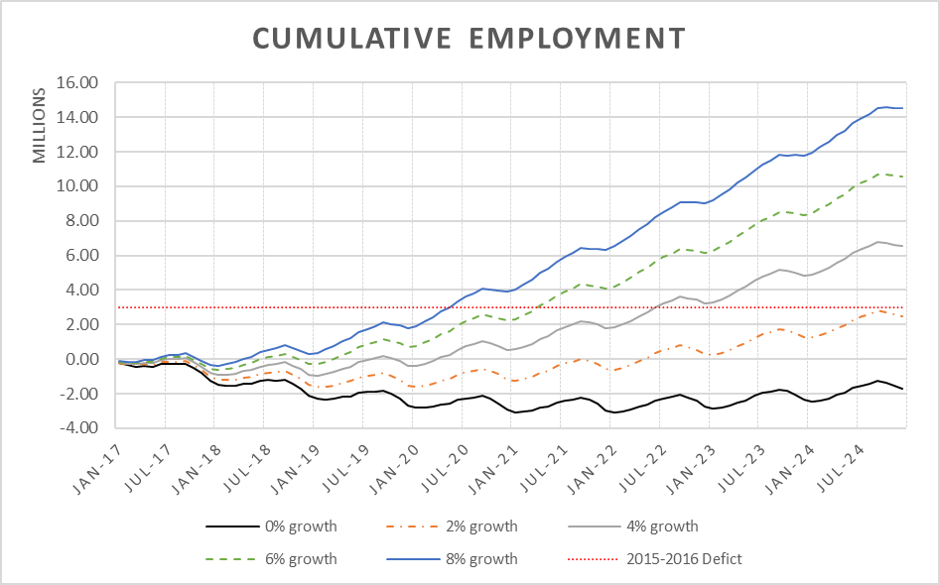
\includegraphics{Figures/Figure1}\tabularnewline
{\footnotesize{}Source: elaborated by the author}\tabularnewline
{\footnotesize{}Note: 2015-2016 deficit: The net employment deficit
accumulated from 2015 through 2016}\tabularnewline
\end{tabular}

\caption{Brazilian accumulated employment forecast for different growth scenarios}
\label{fig: fig-1}
\end{figure}

\begin{figure}
\begin{tabular}{cc}
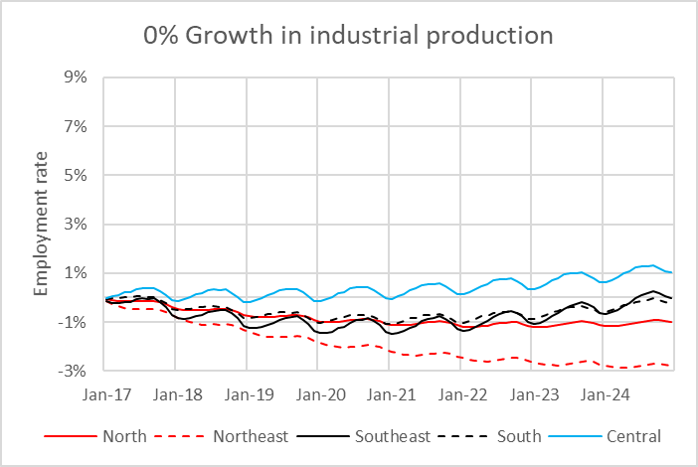
\includegraphics[width=8cm]{Figures/Figure2-a} & 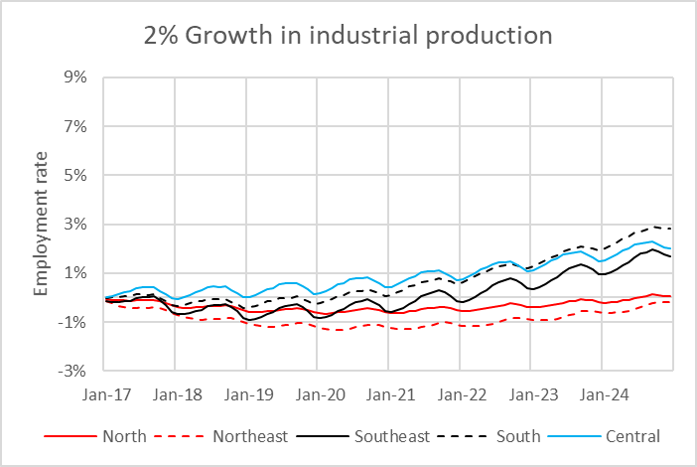
\includegraphics[width=8cm]{Figures/Figure2-b}\tabularnewline
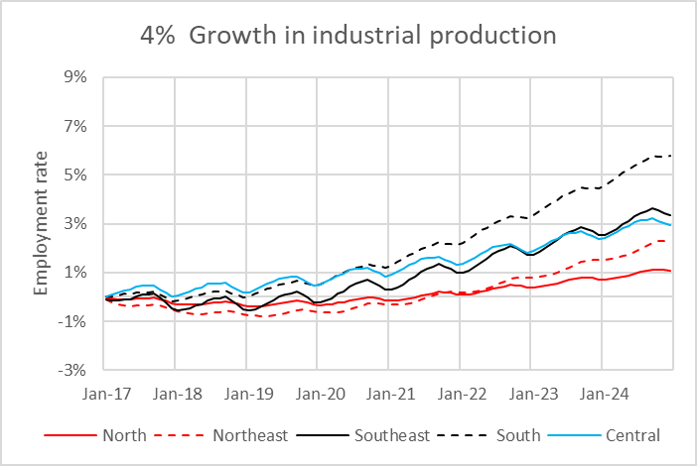
\includegraphics[width=8cm]{Figures/Figure2-c} & 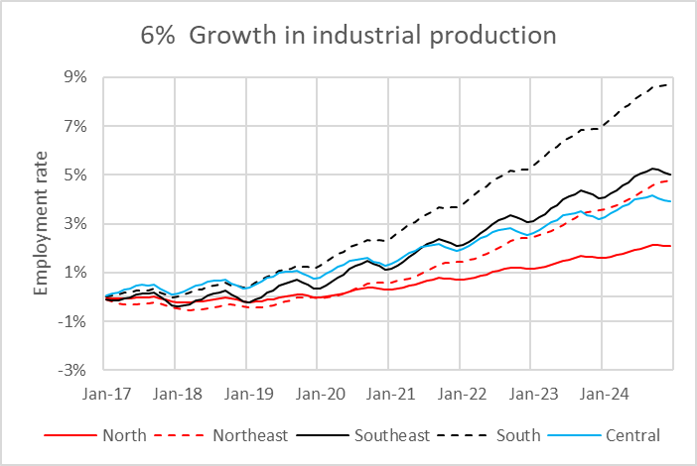
\includegraphics[width=8cm]{Figures/Figure2-d}\tabularnewline
\multicolumn{2}{l}{{\footnotesize{}Source: elaborated by the authors}}\tabularnewline
\end{tabular}

\caption{Accumulated employment rate variation for various industrial production
growth scenarios}
\label{fig: fig-2}
\end{figure}

\begin{figure}
\begin{tabular}{cc}
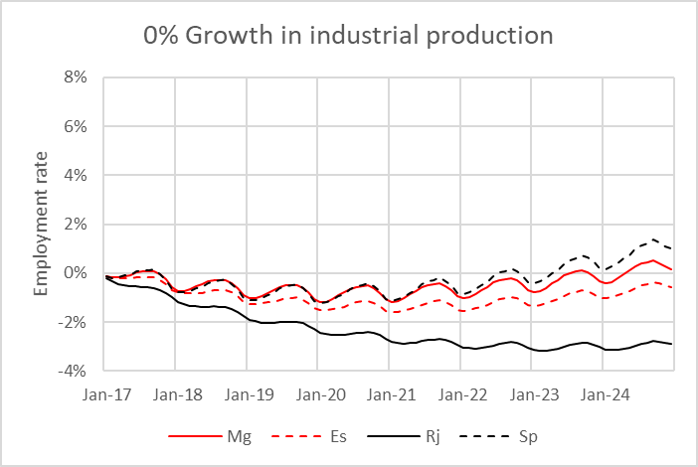
\includegraphics[width=8cm]{Figures/Figure3-a} & 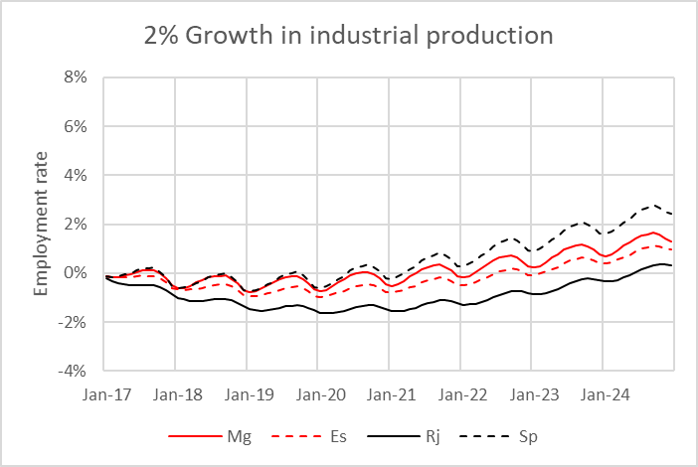
\includegraphics[width=8cm]{Figures/Figure3-b}\tabularnewline
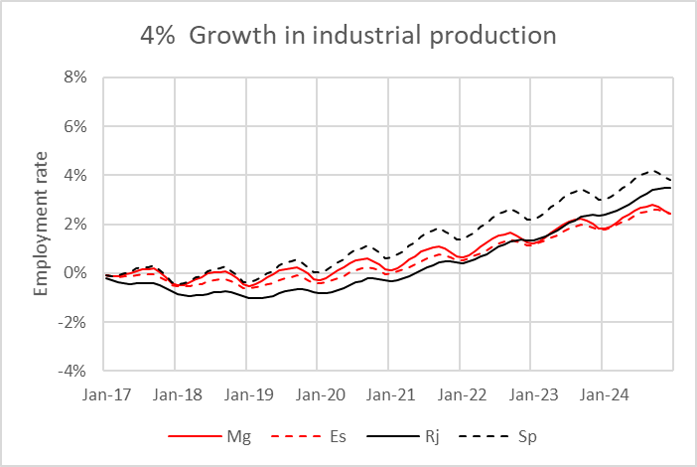
\includegraphics[width=8cm]{Figures/Figure3-c} & 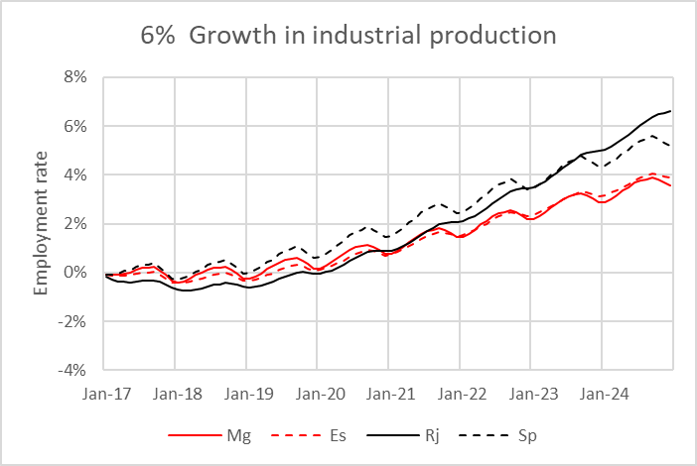
\includegraphics[width=8cm]{Figures/Figure3-d}\tabularnewline
\multicolumn{2}{l}{{\footnotesize{}Source: elaborated by the author}}\tabularnewline
\multicolumn{2}{l}{{\footnotesize{}Mg: Minas Gerais; Es: Esp�rito Santo; Rj: Rio de Janeiro;
Sp: S�o Paulo.}}\tabularnewline
\end{tabular}

\caption{Accumulated employment rate variation for various industrial production
growth scenarios on state level.}
\label{fig: fig-3}
\end{figure}

\begin{figure}
\begin{tabular}{cc}
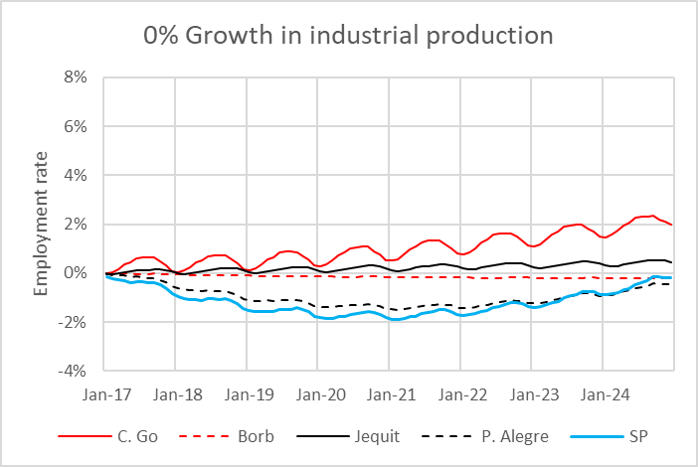
\includegraphics[width=8cm]{Figures/Figure4-a} & 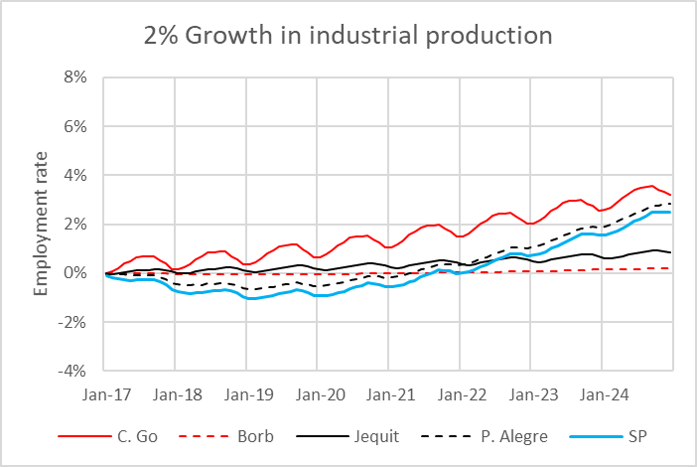
\includegraphics[width=8cm]{Figures/Figure4-b}\tabularnewline
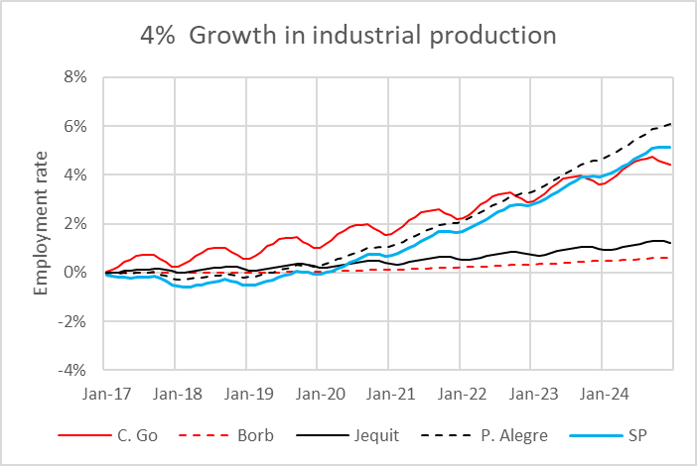
\includegraphics[width=8cm]{Figures/Figure4-c} & 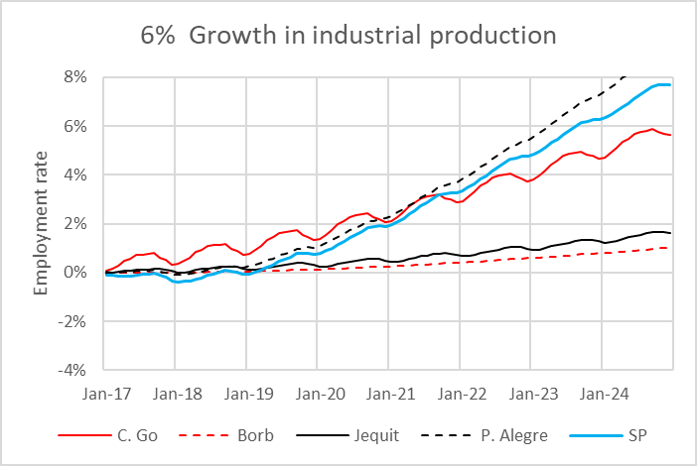
\includegraphics[width=8cm]{Figures/Figure4-d}\tabularnewline
\multicolumn{2}{l}{{\footnotesize{}Source: elaborated by the author }}\tabularnewline
\multicolumn{2}{l}{{\footnotesize{}C.Go: Goi�s central area; Borb: Borborema; Jequit:
Jequitinhonha;}}\tabularnewline
\multicolumn{2}{l}{{\footnotesize{} P.Alegre: Porto Alegre metropolitan area; SP: S�o
Paulo metropolitan area}}\tabularnewline
\end{tabular}
\raggedright{}\caption{Cumulative employment rate changes for various industrial production
growth scenarios on mesoregion level.}
\label{fig: fig-4}
\end{figure}

\begin{figure}
\begin{tabular}{cc}
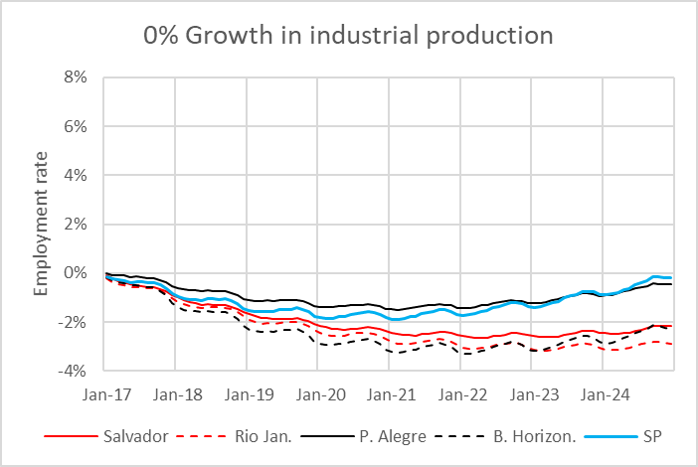
\includegraphics[width=7cm]{Figures/Figure5-a} & 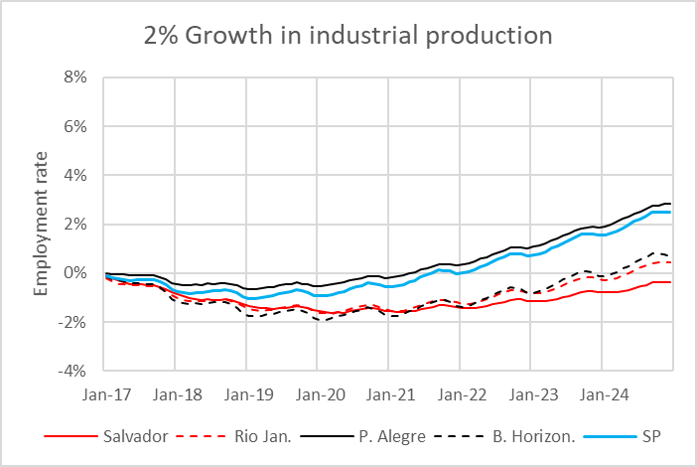
\includegraphics[width=7cm]{Figures/Figure5-b}\tabularnewline
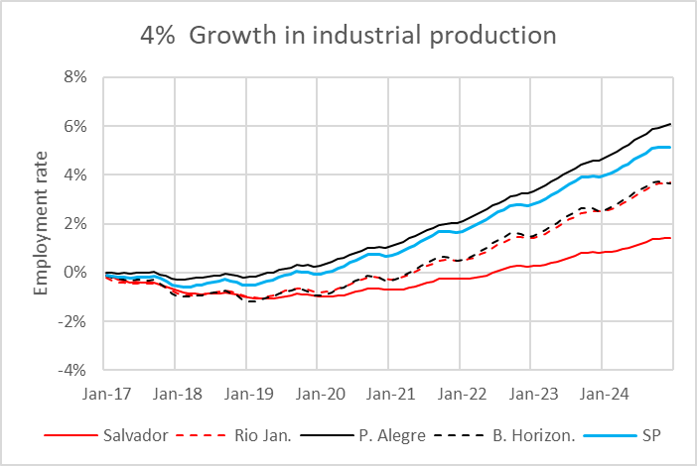
\includegraphics[width=7cm]{Figures/Figure5-c} & 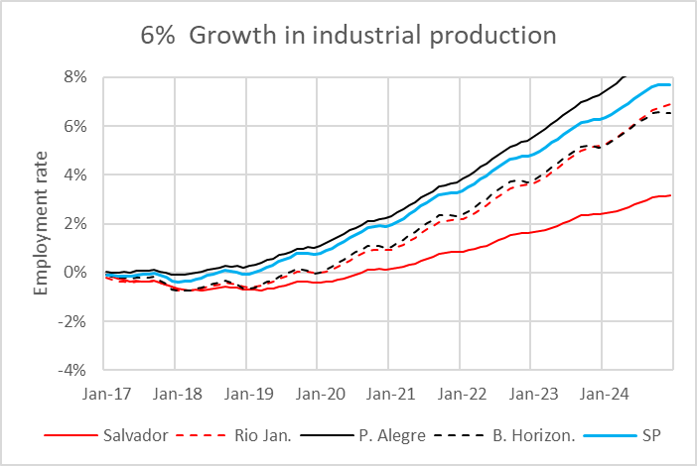
\includegraphics[width=7cm]{Figures/Figure5-d}\tabularnewline
\multicolumn{2}{l}{{\footnotesize{}Source: elaborated by the author }}\tabularnewline
\multicolumn{2}{l}{{\footnotesize{}Salvador: Salvador metropolitan area; Rio Jan: Rio
de Janeiro metropolitan area; }}\tabularnewline
{\footnotesize{}P.Alegre: Porto Alegre metropolitan area;} & \tabularnewline
\multicolumn{2}{l}{{\footnotesize{} B.Horizon.: Belo Horizonte metropolitan area SP:
S�o Paulo metropolitan area}}\tabularnewline
\end{tabular}

\caption{Accumulated employment rate variation for various industrial production
growth scenarios on mesoregion level -- Most populated mesoregions.}
\label{fig: fig-5}
\end{figure}

\begin{figure}
\begin{tabular}{l}
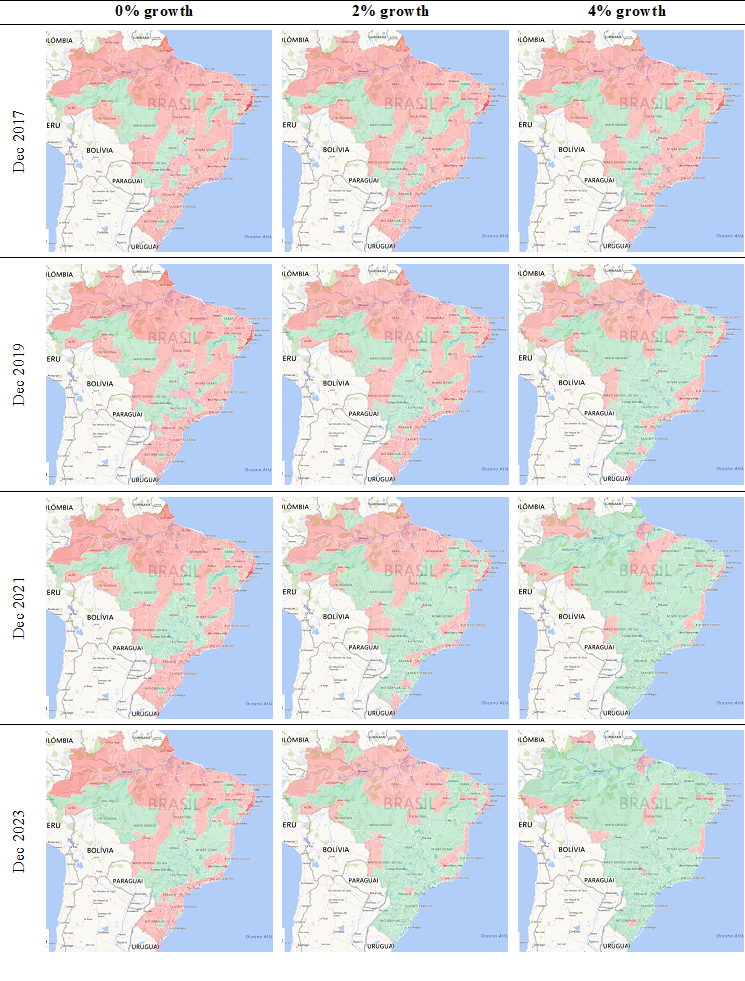
\includegraphics[width=16cm]{Figures/Figure6}\tabularnewline
{\footnotesize{}Source: elaborated by the author. }\tabularnewline
{\footnotesize{}Original data from: CAGED}\tabularnewline
\end{tabular}

\caption{Dynamic comparison of the accumulated employment rate between different
growth scenarios}
\label{fig: fig-6}
\end{figure}

\end{document}
